The course notes use the time convention $e^{-i\omega t}$. With that convention, a forward wave travels in the positive $x$ direction and a backward wave travels in the negative $x$ direction. For A.4.1.a, the two waves with amplitude $1/2$ are

\[\boxed{u^+(x,t)=\frac{1}{2}e^{i(\gamma x-\omega t)},\qquad
u^-(x,t)=\frac{1}{2}e^{-i(\gamma x+\omega t)}}\qquad\text{(A.4.1.a)}\]

Adding these waves and factoring out their common time dependence gives the complex standing-wave expression

\[\boxed{\begin{aligned}
u(x,t)&=u^+(x,t)+u^-(x,t)\\
&=\frac{1}{2}\left(e^{i\gamma x}+e^{-i\gamma x}\right)e^{-i\omega t}\\
&=\cos(\gamma x)e^{-i\omega t}.
\end{aligned}}\qquad\text{(A.4.1.b)}\]

Euler's formula, $\cos(\gamma x)=\tfrac{1}{2}(e^{i\gamma x}+e^{-i\gamma x})$, gives the real trigonometric displacement

\[\boxed{u_{\mathrm{phys}}(x,t)=\Re\{u(x,t)\}=\cos(\gamma x)\cos(\omega t)}\qquad\text{(A.4.1.c)}\]

Its spatial shape stays fixed while its amplitude oscillates in time. The nodes occur where the cosine factor vanishes, and the bows, or antinodes, occur where its magnitude is one.

\textbf{A.4.2. Nodes and antinodes.} The first node is at $x=\lambda/4$ for the cosine phase chosen above. Subsequent nodes are separated by $\lambda/2$, while antinodes lie halfway between adjacent nodes. The figure shows one wavelength and marks both fixed nodes and antinodes.
\begin{figure}[H]
\centering
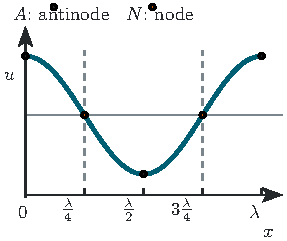
\includegraphics[width=0.55\linewidth]{figures/generated/solutions/A4-standing-wave.pdf}
\caption{A.4.2. Standing-wave displacement shape at an instant. Nodes remain fixed; antinodes reach the maximum displacement.}
\end{figure}

For A.4.3, the input data are
\begin{center}\small
\begin{tabular}{@{}lrl@{}}
\toprule\noalign{}
Quantity & Value & Unit \\
\midrule\noalign{}
$c$ & 340 & m/s \\
$f$ & 2.9 & kHz \\
\bottomrule
\end{tabular}
\end{center}
The frequency and wavespeed give
\[
\omega=2\pi f,\qquad \gamma=\frac{\omega}{c}=\frac{2\pi}{\lambda},\qquad \lambda=\frac{c}{f}.
\]
With $c=340\ \mathrm{m/s}$ and $f=2.9\ \mathrm{kHz}=2900\ \mathrm{Hz}$, the angular frequency and wavenumber are
\[
\begin{aligned}
\omega&=2\pi(2900\ \mathrm{Hz})=18221.2374\ \mathrm{rad/s},\\
\gamma&=\frac{18221.2374\ \mathrm{rad/s}}{340\ \mathrm{m/s}}=53.5919\ \mathrm{rad/m}.
\end{aligned}
\]
These values give the wavelength and node spacing
\[
\lambda=\frac{340\ \mathrm{m/s}}{2900\ \mathrm{Hz}}=0.117241\ \mathrm{m},\qquad
\Delta x=\frac{\pi}{\gamma}=\frac{\lambda}{2}=0.0586207\ \mathrm{m}.
\]
The resulting values are
\[\boxed{\begin{aligned}
\omega&=1.822\times10^4\ \mathrm{rad/s} &&\text{(A.4.3.a)},\\
\gamma&=53.6\ \mathrm{rad/m} &&\text{(A.4.3.b)},\\
\lambda&=0.1172\ \mathrm{m} &&\text{(A.4.3.c)},\\
\Delta x&=0.0586\ \mathrm{m} &&\text{(A.4.3.d)}.
\end{aligned}}\]

\textbf{A.4.4. Taut-string analogy.} A small transverse disturbance on a taut string travels along the string, reflects from a fixed end, and overlaps the returning wave. When the incident and reflected waves have the same frequency and amplitude, their superposition creates fixed points of zero displacement and intervening bows that oscillate in place. Adjacent bows move in opposite directions. The string therefore vibrates as a standing mode even though each component wave propagates. A string fixed at both ends must have a node at each end, so its free standing modes require an integer number of half wavelengths, $L=n\lambda/2$ for $n=1,2,3,\ldots$. The string tension and mass per unit length set the wavespeed and therefore determine the allowed frequencies together with these boundary conditions.

\clearpage
\matlabcaption{MATLAB calculations and standing-wave plot for A.4.}
\lstinputlisting[style=hwmatlab]{matlab/A4.m}
